\subsection{Chèn Tính Kiểm Thử (Testability Insertion)}
Chỉ cần thêm một bộ dẫn tín hiệu, hay một chân input/output, ta đã biến mạch trở nên dễ kiểm thử hơn. Mục này sẽ đề cập đến các lựa chọn cấu trúc phần cứng giúp kiểm thử mạch qua việc điều khiển và quan sát các node.

\begin{figure}[H]
    \centering
    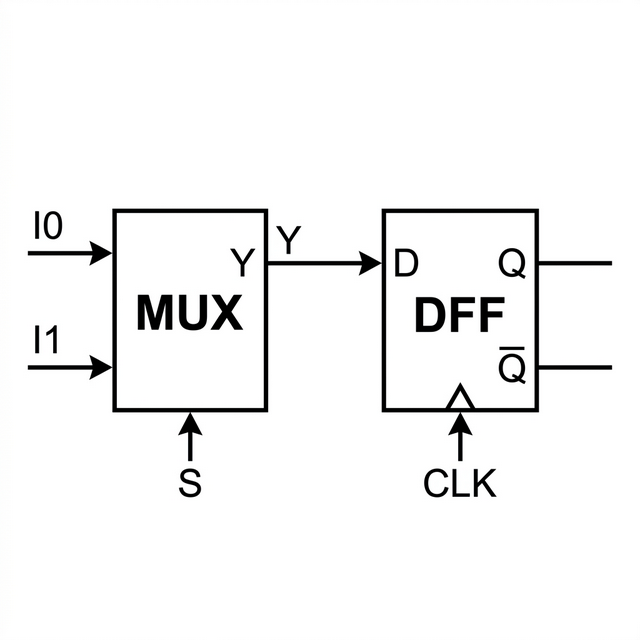
\includegraphics[width=0.7\textwidth]{images/mux_dff.png}
    \caption{\textit{Kỹ thuật kiểm thử cơ bản: khả năng quan sát và điều khiển (Basic testability techniques)}}
\end{figure}

\subsubsection{Cải thiện Khả năng Quan sát (Improving Observability)}
Cải thiện khả năng quan sát giúp hiệu ứng lỗi dễ dàng truyền ra ngoài qua các chân đầu ra sơ cấp thay vì bị kẹt trong mạch. Theo tính toán quan sát (như SCOAP), các đường tín hiệu có độ quan sát thấp nên được nối ra chân ngoài hoặc đưa qua các kỹ thuật như kéo đầu ra flip-flop trạng thái ra thẳng chân output chính.
Trong thiết kế ở mức RTL, các đường cờ điều khiển từ controller sang datapath là những vị trí lý tưởng để quan sát. Trạng thái của multiplexer select, register load, count tín hiệu, v.v. cũng rất phù hợp.

\begin{figure}[H]
    \centering
    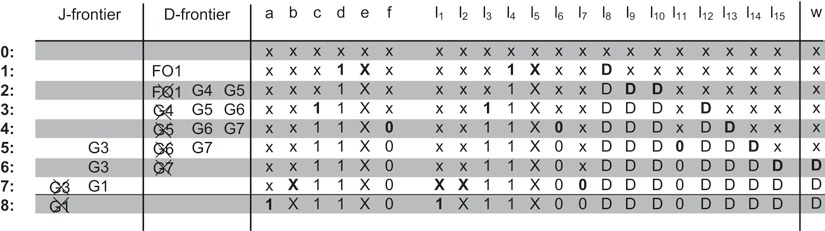
\includegraphics[width=0.7\textwidth]{images/AddingControllability.png}
    \caption{\textit{Cách thêm khả năng điều khiển (Adding controllability)}}
\end{figure}

\subsubsection{Cải thiện Khả năng Điều khiển (Improving Controllability)}
Để tạo tính kiểm thử cho các khối tổ hợp sâu bên trong, ta có thể dùng phần cứng can thiệp vào đường tín hiệu giữa 2 khối logic. Có nhiều kỹ thuật chèn:
\begin{itemize}
    \item \textbf{0-insertion:} Ép một đường dây mang giá trị 0 bằng cấu trúc cổng logic và một chân test.
    \item \textbf{1-insertion:} Ép một đường dây mang giá trị 1 bằng cấu trúc OR gate.
    \item \textbf{0 and 1-insertion:} Cho phép điều khiển chèn cả giá trị 0 lẫn 1 thông qua cấu trúc phức hợp.
    \item \textbf{Test Data Multiplexing (Chèn dữ liệu kiểm thử):} Dùng bộ dồn kênh (MUX) điều khiển bởi tín hiệu \texttt{NbarT}. Khi $\texttt{NbarT} = 0$, mạch ở chế độ thường. Khi $\texttt{NbarT} = 1$, tín hiệu kiểm thử từ input ngoài sẽ được đưa thẳng vào ngõ vào của khối logic cần kiểm tra.
\end{itemize}

\begin{figure}[H]
    \centering
    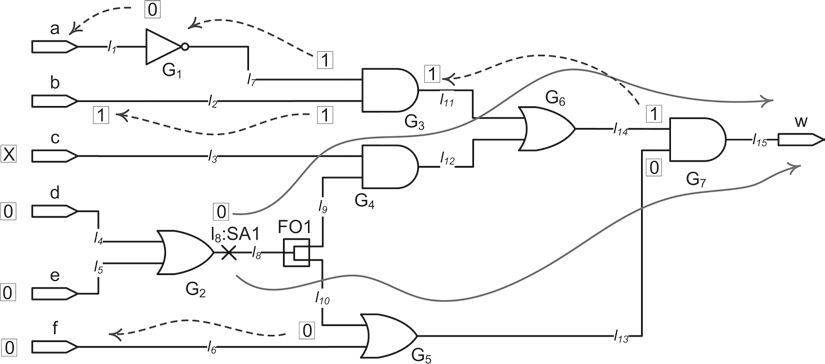
\includegraphics[width=0.7\textwidth]{images/PutCircuitToDesiredState.png}
    \caption{\textit{Đặt mạch vào trạng thái mong muốn (Put circuit into any desired state)}}
\end{figure}

\subsubsection{Chia sẻ Chân Quan sát và Chân Điều khiển}
Việc thêm quá nhiều chân đầu ra hoặc đầu vào sơ cấp là không thực tế. Do đó, mạch sử dụng Multiplexer để dồn nhiều node quan sát vào một chân output duy nhất (cần $\log_2 n$ chân chọn select). Tương tự, một bộ Demultiplexer có thể được dùng để luân phiên điều khiển nhiều đường dây khác nhau (Test point) chỉ với một cổng đầu vào, tiết kiệm $n$ chân kiểm thử.

\begin{figure}[H]
    \centering
    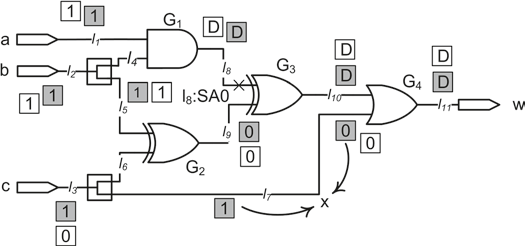
\includegraphics[width=0.7\textwidth]{images/MultiplexingObservation.png}
    \caption{\textit{Kết nối nhiều điểm qua Multiplexer (Multiplexing)}}
\end{figure}

\begin{figure}[H]
    \centering
    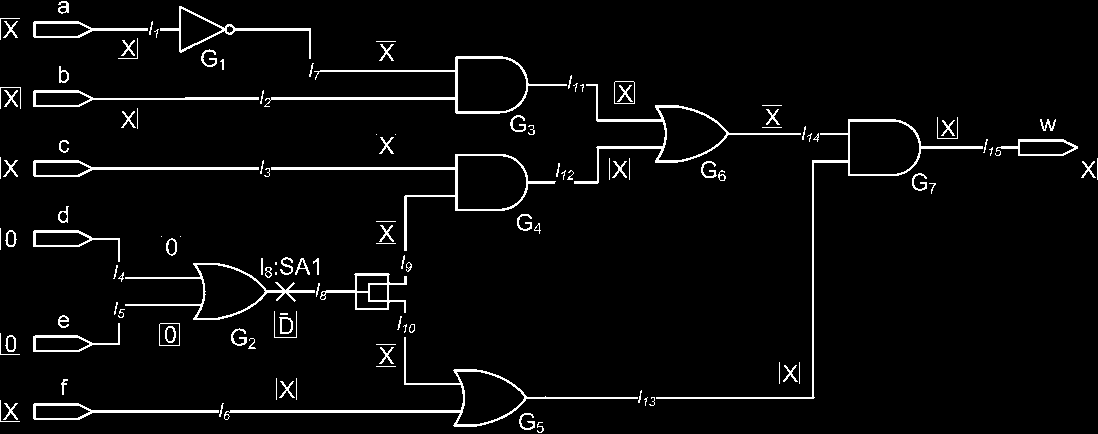
\includegraphics[width=0.7\textwidth]{images/DemultiplexerControl.png}
    \caption{\textit{Dùng Demultiplexer/decoder để giảm số chân (reduce pins for control)}}
\end{figure}

Để tiết kiệm chân select của MUX/DEMUX hơn nữa, một bộ đếm (Counter) có thể được tích hợp trong chip. Chỉ cần cấp xung nhịp cho Counter, nó sẽ tự đếm vòng và chọn các node tương ứng, đổi lấy thời gian kiểm thử dài hơn nhưng không tốn diện tích chân chip.

\begin{figure}[H]
    \centering
    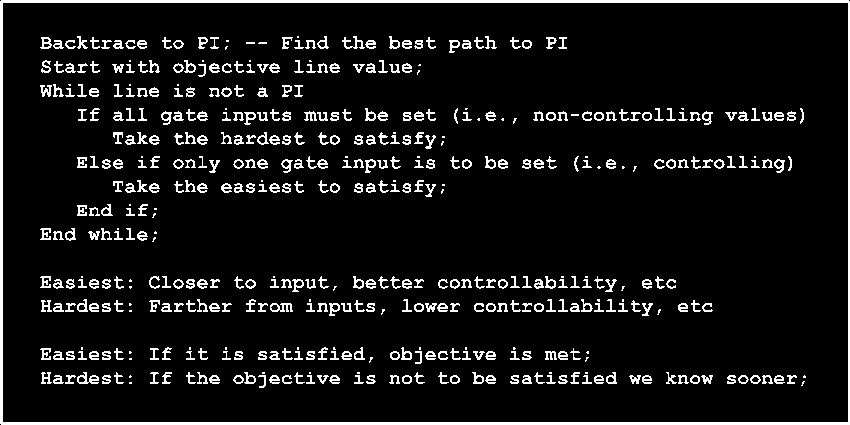
\includegraphics[width=0.7\textwidth]{images/DemultiplexerControlAlternative.png}
    \caption{\textit{Chia sẻ phần cứng chèn trị 1 (Sharing 1-insertion hardware)}}
\end{figure}

\begin{figure}[H]
    \centering
    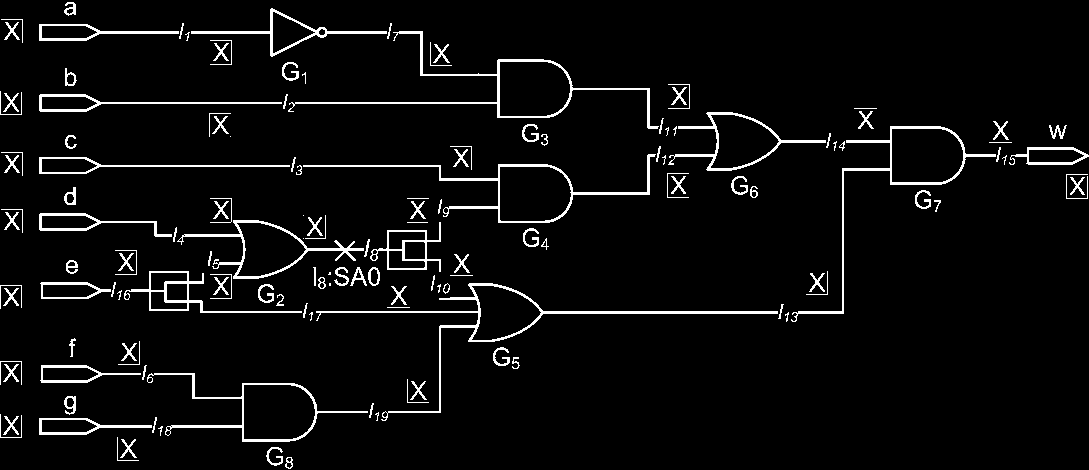
\includegraphics[width=0.7\textwidth]{images/MultiplexersBetweenLogicParts.png}
    \caption{\textit{Chia sẻ phần cứng nạp dữ liệu kiểm thử (Sharing test data insertion hardware)}}
\end{figure}

\subsubsection{Giảm số lượng chân chọn (Reducing Select Inputs)}
Trong một số kiến trúc đặc thù, việc cung cấp đủ số chân Select cho các bộ MUX lớn vẫn là gánh nặng. Kỹ thuật "Reducing Select Inputs" giúp giải quyết bài toán này bằng hai phương án:
\begin{itemize}
    \item \textbf{Decoded Select Lines:} Sử dụng mạch giải mã (Decoder) bên trong chip để mở rộng số chân điều khiển từ một lượng logarit các chân tín hiệu Select bên ngoài. Ví dụ, với 3 chân Select rời, thông qua Decoder $3$-to-$8$, ta điều khiển độc lập được $8$ cấu trúc MUX nội tại.
    \item \textbf{Token Passing:} Chuyền cờ tín hiệu tuần tự qua một thanh ghi dịch (Shift Register). Ở mỗi chu kỳ xung nhịp, chỉ có một cổng logic duy nhất nhận được "Token" kích hoạt trạng thái Test, các cổng còn lại giữ cấu hình mặc định, tiết kiệm đáng kể chi phí định tuyến nối Select song song dọc toàn bộ bề mặt thiết kế.
\end{itemize}

\subsubsection{Điều khiển và Quan sát Đồng thời (Simultaneous Control and Observation)}

\begin{figure}[H]
    \centering
    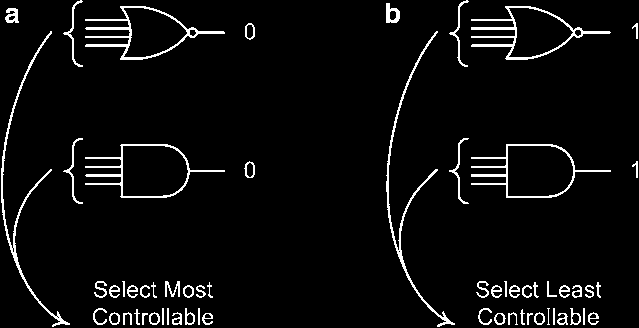
\includegraphics[width=0.7\textwidth]{images/SimultaneousControlBitsOfBuses.png}
    \caption{\textit{Điều khiển đồng thời các bit của Bus (Simultaneous control of bits of buses)}}
\end{figure}

\begin{figure}[H]
    \centering
    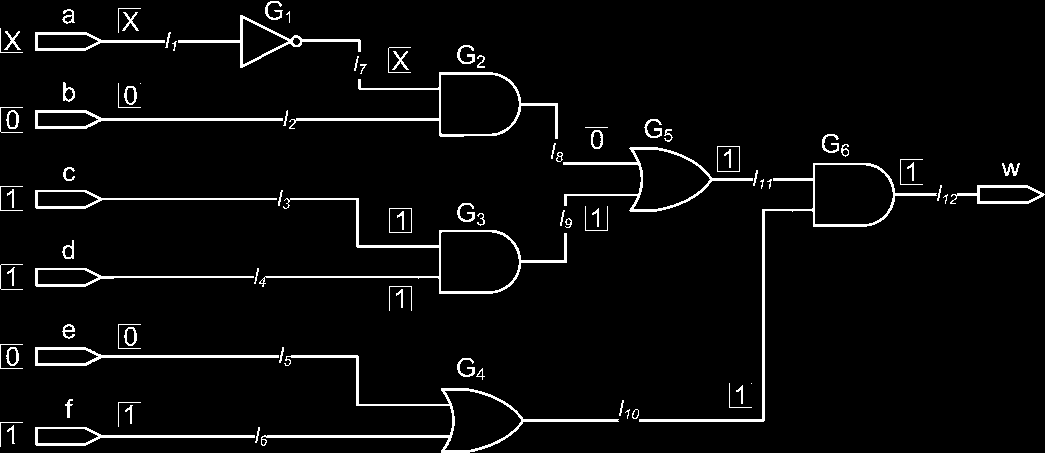
\includegraphics[width=0.7\textwidth]{images/ShiftRegisterSimultaneousControl.png}
    \caption{\textit{Sử dụng Shift-register để điều khiển đồng thời (Shift-register for simultaneous control)}}
\end{figure}

\begin{figure}[H]
    \centering
    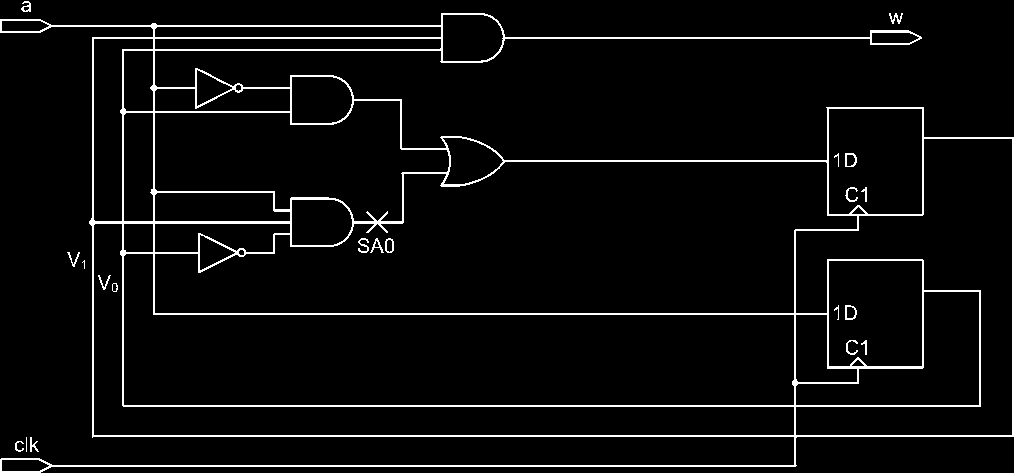
\includegraphics[width=0.7\textwidth]{images/ShiftRegisterSimultaneousCollection.png}
    \caption{\textit{Sử dụng thanh ghi dịch để thu thập đồng thời (Using a shift-register for simultaneous collection)}}
\end{figure}

Để điều khiển các tín hiệu đồng thời với số chân hạn chế, kỹ thuật thanh ghi dịch (Shift Register) được áp dụng để tải nối tiếp dữ liệu sau đó xuất song song vào các điểm kiểm thử. Tương tự đối với thu thập đầu ra: thu song song và dịch nối tiếp ra ngoài.
\paragraph{Isolated Serial Scan} kết hợp hai thao tác trên vào chung một thanh ghi dịch. Thanh ghi này cô lập khỏi luồng điều khiển chính qua tín hiệu phân vùng \texttt{NbarT}, vừa dịch dữ liệu kiểm thử vào, vừa nhận phản hồi và dịch ra trong suốt một số chu kỳ kiểm thử.  

\begin{figure}[H]
    \centering
    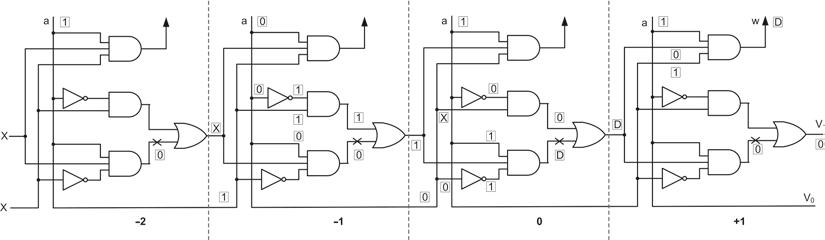
\includegraphics[width=0.7\textwidth]{images/IsolatedSerialScan.png}
    \caption{\textit{Quét nối tiếp cô lập (Isolated Serial Scan)}}
\end{figure}

\begin{figure}[H]
    \centering
    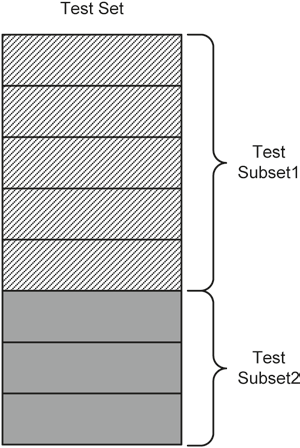
\includegraphics[width=0.7\textwidth]{images/IsolatedSerialScanShiftRegister.png}
    \caption{\textit{Thanh ghi dịch cho Isolated Serial Scan}}
\end{figure}

\begin{lstlisting}[language=Verilog, caption={Mã giả Verilog cho hệ thống Isolated Serial Scan (Shift-register)}]
module shiftreg #(parameter size = 4) (
    input [size-1:0] parin, 
    input TestClock, SerialTestDataIn, 
    input [1:0] TestMode,
    output SerialTestDataOut,
    output reg [size-1:0] parout
);
    always @(posedge TestClock) begin
        case (TestMode) 
            0: parout <= parout;          
            1: parout <= {SerialTestDataIn, parout[size-1:1]}; // Shift mode
            2: parout <= parin; // Parallel load
            3: parout <= 0;     // Reset
        endcase    
    end 
    assign SerialTestDataOut = parout[0]; 
endmodule
\end{lstlisting}

\begin{figure}[H]
    \centering
    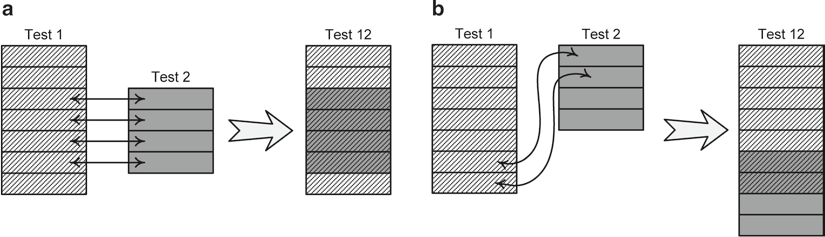
\includegraphics[width=0.7\textwidth]{images/IsolatedSerialScanVirtualTester.png}
    \caption{\textit{Thiết bị thử nghiệm ảo cho Isolated Serial Scan (Virtual tester)}}
\end{figure}

\subsubsection{Khái niệm cơ bản về Thiết kế Quét (Basic concept of SCAN design)}
Như đã nhận thấy ở phần quét nối tiếp cô lập, ý tưởng cốt lõi của Thiết kế Quét (SCAN Design) là thay thế tất cả (hoặc một phần) các bộ nhớ Flip-Flop nội tại trong chip bằng các Scan Flip-Flop (SFF) và kết nối chúng thành các thanh ghi dịch nối tiếp (Shift Register) hay còn gọi là chuỗi quét (Scan Chain). 

Mạch sẽ hoạt động qua hai chế độ song song được khai thác:
\begin{itemize}
    \item \textbf{Chế độ thường (Normal Mode):} Các Flip-Flop đóng vai trò thu thập tín hiệu logic từ mạch và lưu trạng thái bình thường phục vụ chức năng hệ thống.
    \item \textbf{Chế độ quét (Shift/Scan Mode):} Các Flip-Flop tạm thời gạt bỏ luồng dữ liệu thông thường để liên kết thành dây chuyền dịch. Việc này cho phép thiết bị kiểm thử bên ngoài (ATE) trực tiếp dịch (Shift) chuỗi dữ liệu đầu vào (Controllability) hoặc đẩy toàn bộ trạng thái hiện hữu đang được chụp trích ra ngoài nhằm phân tích (Observability).
\end{itemize}

\paragraph{Công cụ tự động hóa (SCAN Tools)}
Quá trình nâng cấp từ hệ thống thường sang hệ thống thiết kế SCAN (ví dụ như thay loại Flip-Flop, định tuyến xung nhịp Scan Clock hay kết nối chân tín hiệu Scan Enable) được thực hiện hoàn toàn tự động bởi các phần mềm phân tích hiện đại. Các công cụ EDA (Electronic Design Automation) phổ biến như Synopsys DFT Compiler hay Mentor Tessent cho phép kỹ sư cấu hình luật vận hành, tự động đánh giá và tối ưu hóa diện tích/hiệu suất (Overhead Rules) mà không cần cấu trúc mạch thủ công phức tạp.
